\textit{Autonomous Intelligent Cyberdefense Agents}~\cite{Kott2023} (AICA) are agents to be deployed in networked environments to detect, identify, and characterize anomalies/attacks, develop countermeasures, and execute them
%
\footnote{
    Theorized by the \textit{AICA International Work Group} (cf. \url{https://www.aica-iwg.org/}) and based on the results of NATO's \textit{Research Task Group IST-152}.
}.
Related AICA research highlights the increasing need for \textit{Autonomous Cyberdefense} to protect decentralized environments where traditional centralized approaches are ineffective, such as in IoT-based systems. A Multi-Agent System (MAS) offers robust and adaptive defense mechanisms by decomposing the complexity of Cyberdefense into sub-tasks delegated to collaborative agents deployed throughout the system.

The top-down approach involves designing Cyberdefense MAS from predefined architectures and functionalities. The \textit{MAS Centric AICA Reference Architecture} (MASCARA)~\cite{Kott2023} describes an AICA-like MAS with components that enable collaborative mechanisms based on explicitly defined plans or processes. However, this approach can be costly as it requires comprehensive knowledge of the deployment environment, which must be regularly updated due to frequent changes, such as topology modifications or new vulnerabilities.

The bottom-up approach may include Multi-Agent Reinforcement Learning (MARL)~\cite{Albrecht2024}, where agents learn to achieve Cyberdefense goals autonomously, enhancing MAS autonomy~\cite{hammar_stadle4_noms_23}. Despite promising simulation results, this approach lacks the safety guarantees necessary for real-world applications and does not provide explicit means to justify the MAS's success or failure~\cite{dulacarnold2019}. These issues hinder the development of fully or semi-autonomous Cyberdefense MAS, such as AICA, in critical environments, where actions must be justified given their potentially irreversible consequences.

To address this concern, we propose combining these two points of view by extending the \textit{Partial Relation between Agents' History and Organizational Model}~\cite{soule2024} (PRAHOM). PRAHOM is a general approach that enables integrating the $\mathcal{M}OISE^+$ organizational model into the MARL framework, laying the foundation for constraining learning. However, this perspective remains limited in its implementation and faces scalability issues with the number of organizational specifications, which limits its application in complex networked environments.

The main contribution of this paper is the \textit{Cyberdefense-oriented PRAHOM} (CoPRAHOM) inspired by PRAHOM and related works. This algorithm is specifically intended to address Cyberdefense scenarios relying on general Cyberdefense architectures such as MASCARA. This algorithm enables users to constrain agents to Cyberdefense roles and missions. We implemented practical means to apply CoPRAHOM also aiming to address scalability concerns. One of the main interests is to ensure safety guarantees by embedding domain-specific knowledge, such as rules, or accelerating or stabilizing the training by restricting the search space.

We assessed CoPRAHOM in the simulated scenario provided by the 3rd CAGE Challenge~\cite{cage_challenge_3_announcement}. It involves creating a Cyberdefense MAS for detecting, mitigating, and eliminating malware programs in a drone swarm. Using CoPRAHOM, we developed several Cyberdefense MAS models. These models are used by CoPRAHOM to guide and constrain agents' training to better achieve the scenario's goals and ensure safety requirements. We verify that the trained agents exhibit expected collective strategies while being also fine-tuned throughout the training, making the overall score comparable to leading entries on the leaderboard.


\subsection{MARL Background}\label{sec:marl_background}

Multi-Agent Reinforcement Learning (MARL) extends the principles of Reinforcement Learning (RL) to scenarios involving multiple interacting agents. Agents aim to maximize the overall cumulative reward through learning, but the presence of other agents introduces additional complexity due to the dynamic nature of the environment.

MARL is often modeled using the Decentralized Partially Observable Markov Decision Process (Dec-POMDP)~\cite{Beynier2013}, a framework suitable for environments where agents have limited and differing observations. A Dec-POMDP is formally defined as a tuple $(S, \{A_i\}, T, R, \{\Omega_i\}, O, \gamma)$:

\begin{itemize}
    \item $S$: A finite set of states describing the environment.
    \item $\{A_i\}$: A set of action sets, one for each agent $i$.
    \item $T$: The state transition probability function $T(s, \vec{a}, s') = P(s'|s, \vec{a})$, where $\vec{a}$ is the joint action of all agents.
    \item $R$: The reward function $R(s, \vec{a}, s')$, mapping states and actions to a reward.
    \item $\{\Omega_i\}$: A set of observation sets, one for each agent $i$.
    \item $O$: The observation probability function $O(\vec{o} | s', \vec{a})$, where $\vec{o}$ is the joint observation of all agents.
    \item $\gamma \in [0,1]$: The discount factor for future rewards.
\end{itemize}

In MARL, each agent $i$ maintains a policy $\pi_i: H \times \Omega \rightarrow A$, mapping an action $a \in A$ from an observation $\omega \in \Omega$ and optionally the agent's history $h \in H, h=\langle(\omega_0,a_0),(\omega_1,a_1)\dots(\omega_{n_e},a_{n_e})\rangle$ (with $n_e \in \mathbb{N}$, the number of steps per episode). A joint policy $\pi_{\text{joint}} = (\pi_1, \pi_2, \ldots, \pi_n)$ describes the behavior of all agents collectively.

The ultimate goal is to find a joint policy $\pi_{\text{joint}}$ that maximizes the expected cumulative reward $U(\pi^*_{\text{joint}}) = \mathbb{E}\left[\sum_{t=0}^{\infty} \gamma^t R(s_t, \vec{a}_t)\right]$. Instead of solely aiming for a global optimum, our approach emphasizes obtaining approximate solutions with sufficient reward.

Various methods have been proposed to address the challenges of MARL.
%
\textbf{Value-based methods}, such as QMIX~\cite{rashid2018}, estimate the value function $Q(s,\vec{a})$, which represents the expected cumulative reward for a given state $s$ and joint action $\vec{a}$. While these methods have shown promising results in simple scenarios, they often struggle to effectively utilize multi-agent communication to enhance overall rewards~\cite{oroojlooy2021review}.
%
\textbf{Policy-based methods}, including Multi-Agent Proximal Policy Optimization (MAPPO)\cite{yu2022surprising} and Multi-Agent Deep Deterministic Policy Gradient (MADDPG)\cite{lowe2017multi}, directly parameterize the policy as $\pi_\theta$ and optimize it, potentially using centralized training with decentralized execution. We have preferred these methods because they have demonstrated significant efficiency in various cooperative and competitive multi-agent contexts~\cite{yu2022surprising}\cite{lowe2017multi}.
%
Lastly, \textbf{Actor-Critic methods} combine value-based and policy-based approaches. For instance, in COMA (Counterfactual Multi-Agent Policy Gradients), the actor updates the policy parameters in the direction indicated by the critic, which evaluates the current policy. Although these methods have proven efficient in single-agent settings, additional efforts are needed to fully adapt them to multi-agent scenarios, particularly in managing the complexity introduced by agents' mutual influence~\cite{papoudakis2021agent}.


\subsection{Related Works}
\label{sec:related_works}

We define organizational-oriented MARL as the broad field of research encompassing studies that introduce explicit specifications (such as rules, roles, or protocols) to guide or restrict the MARL training process to meet requirements. While the explicit integration of organizational specifications in MARL is not extensively covered in the literature, several approaches have been proposed to embed some constraints within MAS to ensure that agents conform to specific requirements.

\textbf{Learning with Organizational Constraints} \quad
In \cite{cruz2020norms}, the authors present a method for incorporating norms into the learning algorithms of agents, ensuring that their behavior remains within acceptable bounds. Additionally, \cite{villatoro2011social} proposes a mechanism for agents to learn and adapt to social norms in dynamic environments, highlighting the importance of norm adaptation in MAS.
%
A relevant subset of work belongs to \emph{Specification-Guided Reinforcement Learning}, which aims to generate policies that accomplish specific tasks using external specifications to guide learning in achieving objectives under given constraints~\cite{Bansal2022}. Jothimurugan et al.~\cite{Jothimurugan2021} propose logical specification learning, exploiting the compositional structure of specifications to generate policies for complex tasks. However, it does not completely fall into the MARL framework we set for it requires introducing logical specifications.

\textbf{MARL in Cybersecurity and Autonomous Cyber Operations} \quad
MARL has also been applied in cybersecurity to develop autonomous systems capable of defending against cyber threats. Albrecht et al.~\cite{Albrecht2024} explore the use of MARL for training agents in dynamic environments to achieve cybersecurity goals.
As previously stated in Kott et al.~\cite{Kott2023}, some works involved by AICAs include the development of simulation frameworks for hand-tailored training of autonomous agents in a decentralized environment~\cite{Drasar2020}.
Similarly, in \cite{Hammar2022}, the authors present a framework using \emph{system identification} methods for integrating digital twins with MARL to enhance cybersecurity automation and enhance MARL applicability in real systems.

\textbf{Policy-Based Approaches} \quad
Some works related to policy-based approaches foster ways to enforce organizational constraints by defining explicit policies that govern agent behavior. In \cite{krupanski2015norm}, the use of normative policies is investigated to guide agent interactions and decision-making processes. Moreover, \cite{vos2020governing} explores the use of governance mechanisms to enforce compliance with organizational policies in decentralized systems. However, these approaches face a lack of practicality in their use and may be difficult to explain since most policies are black-box and cannot be easily modified.

\textbf{Frameworks Integrating Organizational Aspects} \quad
Wang et al.~\cite{Wang2020} introduce an approach in which similar emerging roles are encouraged to jointly specialize in specific tasks. Tosic et al.~\cite{Tosic2010} propose a framework for coordination based on the communication capabilities of multi-agent systems. Zheng et al.~\cite{Zheng2018} present a platform for MARL that aims to facilitate research on artificial collective intelligence by providing a comprehensive set of evaluation metrics to compare the performance of MARL algorithms. However, it does not take into account specifications likely to entice agents to adhere to an expected behavior such as missions.


Despite these advancements, there is still a scarcity of research explicitly utilizing organizational specifications to constrain agent learning in accordance with requirements. To our knowledge, no existing work facilitates the generation of a MAS that explicitly satisfies additional organizational constraints. CoPRAHOM's originality lies in using an organizational model explicitly as a general way for constraining learning based on these requirements.

\subsection{Combining $\mathcal{M}OISE^+$ Model with MARL}
\label{sec:marl_moise_linking}

This section briefly presents the principles we propose for adapting MARL with organizational specifications to align policies with expected role behaviors and mission goals.

The $\mathcal{M}OISE^+$ model provides a structured framework for defining roles and interactions within a Multi-Agent System (MAS). It is compatible with MARL, allowing for formal descriptions of agent policies. The CoPRAHOM approach embeds $\mathcal{M}OISE^+$ specifications into MARL training, enabling agents to adhere to predefined roles and missions. $\mathcal{M}OISE^+$ defines \textbf{Organizational Specifications (OS)} as $\mathcal{OS} = \langle \mathcal{SS}, \mathcal{FS}, \mathcal{DS} \rangle$, where $\mathcal{SS}$ are \textbf{Structural Specifications}, $\mathcal{FS}$ are \textbf{Functional Specifications}, and $\mathcal{DS}$ are \textbf{Deontic Specifications}.

\subsubsection{Structural Specifications}

\textbf{Structural Specifications} ($\mathcal{SS} = \langle \mathcal{R}, \mathcal{IR}, \mathcal{G} \rangle$) describe organizational structure:
\begin{itemize}
    \item $\mathcal{R}_{ss}$: All roles ($\rho \in \mathcal{R}$).
    \item $\mathcal{IR}$: Role inheritance relation ($\rho_1 \sqsubset \rho_2$).
    \item $\mathcal{RG} \subseteq \mathcal{GR}$: Root groups, $\mathcal{GR} = \langle \mathcal{R}, \mathcal{SG}, \mathcal{L}^{intra}, \mathcal{L}^{inter}, \mathcal{C}^{intra}, \mathcal{C}^{inter}, np, ng \rangle$, where:
          \begin{itemize}
              \item $\mathcal{R}$: Non-abstract roles.
              \item $\mathcal{SG}$: Sub-groups.
              \item $\mathcal{L}^{intra}$ and $\mathcal{L}^{inter}$: Intra and inter group links denoted as a 3-tuple $(\rho_s, \rho_d, t)$, where $t \in \{acq, com, aut\}$.
              \item $\mathcal{C}^{intra}$ and $\mathcal{C}^{inter}$: Intra and inter group compatibilities denoted as $\rho_a \bowtie \rho_b$.
              \item $np$: Cardinality of agents in a role.
              \item $ng$: Cardinality of each sub-group.
          \end{itemize}
\end{itemize}

Direct policy constraints are impractical due to black-box models like neural networks. Instead, we represent roles as history subsets $\mathcal{P}(H)$ that agents should generate, characterizing expected behaviors. Each role maps to a history subset via $rh: \mathcal{R} \rightarrow \mathcal{P}(H)$. Agents' policies should generate histories belonging to these subsets.

We address large, complex observations by using labels to represent observations. The mapping $ol: \mathcal{P}(\Omega) \rightarrow \mathcal{P}(L)$ translates observations to labels, potentially using a trained Large Language Model (LLM). This simplifies defining history subsets, which can be represented by patterns, rules, or custom scripts.

\begin{figure}[h!]
    \centering
    


\tikzset{every picture/.style={line width=0.75pt}} %set default line width to 0.75pt        

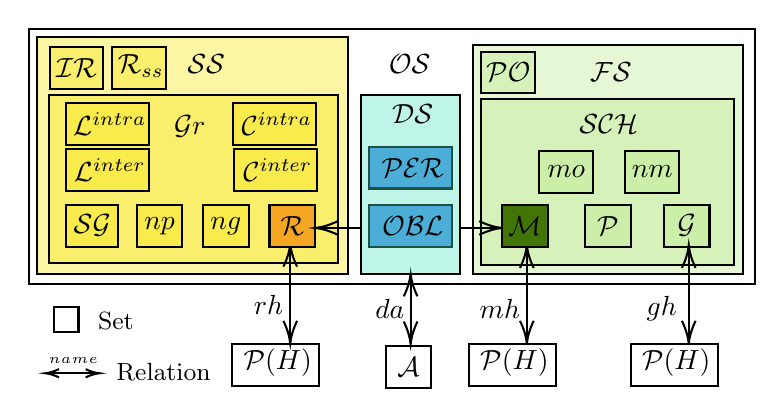
\begin{tikzpicture}[x=0.75pt,y=0.75pt,yscale=-1,xscale=1]
%uncomment if require: \path (0,1800); %set diagram left start at 0, and has height of 1800

%Shape: Rectangle [id:dp9341453924522656] 
\draw  [fill={rgb, 255:red, 255; green, 255; blue, 255 }  ,fill opacity=1 ] (160,44) -- (510,44) -- (510,167) -- (160,167) -- cycle ;
%Shape: Rectangle [id:dp4628140741854456] 
\draw  [fill={rgb, 255:red, 184; green, 233; blue, 134 }  ,fill opacity=0.34 ] (374,52) -- (504,52) -- (504,162) -- (374,162) -- cycle ;
%Shape: Rectangle [id:dp6461749357206974] 
\draw  [fill={rgb, 255:red, 184; green, 233; blue, 134 }  ,fill opacity=0.34 ] (378,78) -- (500,78) -- (500,158) -- (378,158) -- cycle ;
%Shape: Rectangle [id:dp47018118728898073] 
\draw  [fill={rgb, 255:red, 248; green, 231; blue, 28 }  ,fill opacity=0.4 ] (164,48) -- (314,48) -- (314,162) -- (164,162) -- cycle ;
%Straight Lines [id:da37904402438854] 
\draw    (400,150.31) -- (400,193.69) ;
\draw [shift={(400,195.69)}, rotate = 270] [color={rgb, 255:red, 0; green, 0; blue, 0 }  ][line width=0.75]    (10.93,-3.29) .. controls (6.95,-1.4) and (3.31,-0.3) .. (0,0) .. controls (3.31,0.3) and (6.95,1.4) .. (10.93,3.29)   ;
\draw [shift={(400,148.31)}, rotate = 90] [color={rgb, 255:red, 0; green, 0; blue, 0 }  ][line width=0.75]    (10.93,-3.29) .. controls (6.95,-1.4) and (3.31,-0.3) .. (0,0) .. controls (3.31,0.3) and (6.95,1.4) .. (10.93,3.29)   ;
%Straight Lines [id:da30557994145553513] 
\draw    (368,140) -- (386,140) ;
\draw [shift={(388,140)}, rotate = 180] [color={rgb, 255:red, 0; green, 0; blue, 0 }  ][line width=0.75]    (10.93,-3.29) .. controls (6.95,-1.4) and (3.31,-0.3) .. (0,0) .. controls (3.31,0.3) and (6.95,1.4) .. (10.93,3.29)   ;
%Shape: Rectangle [id:dp15689957472567295] 
\draw  [fill={rgb, 255:red, 248; green, 231; blue, 28 }  ,fill opacity=0.4 ] (169.56,76) -- (309.06,76) -- (309.06,157) -- (169.56,157) -- cycle ;
%Shape: Rectangle [id:dp6202366628126772] 
\draw  [fill={rgb, 255:red, 255; green, 255; blue, 255 }  ,fill opacity=1 ] (372,196) -- (414,196) -- (414,216) -- (372,216) -- cycle ;

%Shape: Rectangle [id:dp20067598884831228] 
\draw  [fill={rgb, 255:red, 248; green, 231; blue, 28 }  ,fill opacity=0.4 ] (212.06,129) -- (234.06,129) -- (234.06,149) -- (212.06,149) -- cycle ;

%Shape: Rectangle [id:dp5970765798398485] 
\draw  [fill={rgb, 255:red, 248; green, 231; blue, 28 }  ,fill opacity=0.4 ] (178.06,129) -- (203.06,129) -- (203.06,149) -- (178.06,149) -- cycle ;
%Shape: Rectangle [id:dp92237875722883] 
\draw  [fill={rgb, 255:red, 248; green, 231; blue, 28 }  ,fill opacity=0.4 ] (178.06,102) -- (218.06,102) -- (218.06,122) -- (178.06,122) -- cycle ;

%Shape: Rectangle [id:dp6591761395302378] 
\draw  [fill={rgb, 255:red, 248; green, 231; blue, 28 }  ,fill opacity=0.4 ] (178.06,80) -- (218.06,80) -- (218.06,100) -- (178.06,100) -- cycle ;

%Shape: Rectangle [id:dp11794703752595392] 
\draw  [fill={rgb, 255:red, 248; green, 231; blue, 28 }  ,fill opacity=0.4 ] (258.5,80) -- (298.5,80) -- (298.5,100) -- (258.5,100) -- cycle ;

%Shape: Rectangle [id:dp6557958558103134] 
\draw  [fill={rgb, 255:red, 248; green, 231; blue, 28 }  ,fill opacity=0.4 ] (259,102) -- (299,102) -- (299,122) -- (259,122) -- cycle ;

%Shape: Rectangle [id:dp8284992701408749] 
\draw  [fill={rgb, 255:red, 65; green, 117; blue, 5 }  ,fill opacity=1 ] (388,129) -- (410,129) -- (410,149) -- (388,149) -- cycle ;

%Shape: Rectangle [id:dp7066110016250453] 
\draw  [fill={rgb, 255:red, 248; green, 231; blue, 28 }  ,fill opacity=0.4 ] (244,129) -- (266,129) -- (266,149) -- (244,149) -- cycle ;

%Shape: Rectangle [id:dp4021333114319714] 
\draw  [fill={rgb, 255:red, 248; green, 231; blue, 28 }  ,fill opacity=0.4 ] (170.31,53) -- (195.69,53) -- (195.69,73) -- (170.31,73) -- cycle ;

%Shape: Rectangle [id:dp8476756388266236] 
\draw  [fill={rgb, 255:red, 248; green, 231; blue, 28 }  ,fill opacity=0.4 ] (200,53) -- (226,53) -- (226,73) -- (200,73) -- cycle ;

%Shape: Rectangle [id:dp07470576340681823] 
\draw  [fill={rgb, 255:red, 74; green, 144; blue, 226 }  ,fill opacity=1 ] (324,101) -- (364,101) -- (364,121) -- (324,121) -- cycle ;

%Shape: Rectangle [id:dp31407652093057714] 
\draw  [fill={rgb, 255:red, 74; green, 144; blue, 226 }  ,fill opacity=1 ] (324,129) -- (364,129) -- (364,149) -- (324,149) -- cycle ;

%Shape: Rectangle [id:dp053729126169398844] 
\draw  [fill={rgb, 255:red, 184; green, 233; blue, 134 }  ,fill opacity=0.34 ] (378,55) -- (404,55) -- (404,75) -- (378,75) -- cycle ;

%Shape: Rectangle [id:dp7720103442630182] 
\draw  [fill={rgb, 255:red, 184; green, 233; blue, 134 }  ,fill opacity=0.34 ] (405.94,103) -- (431.94,103) -- (431.94,123) -- (405.94,123) -- cycle ;

%Shape: Rectangle [id:dp3183552657000306] 
\draw  [fill={rgb, 255:red, 184; green, 233; blue, 134 }  ,fill opacity=0.34 ] (447.44,103) -- (473.44,103) -- (473.44,123) -- (447.44,123) -- cycle ;

%Shape: Rectangle [id:dp10802424702469593] 
\draw  [fill={rgb, 255:red, 184; green, 233; blue, 134 }  ,fill opacity=0.34 ] (466,129) -- (488,129) -- (488,149) -- (466,149) -- cycle ;

%Shape: Rectangle [id:dp16589412198505937] 
\draw  [fill={rgb, 255:red, 184; green, 233; blue, 134 }  ,fill opacity=0.34 ] (428,129) -- (450,129) -- (450,149) -- (428,149) -- cycle ;

%Shape: Rectangle [id:dp1270989692188249] 
\draw  [fill={rgb, 255:red, 255; green, 255; blue, 255 }  ,fill opacity=1 ] (258,196) -- (300,196) -- (300,216) -- (258,216) -- cycle ;

%Straight Lines [id:da40017392935840324] 
\draw    (286,149.69) -- (286,193.69) ;
\draw [shift={(286,195.69)}, rotate = 270] [color={rgb, 255:red, 0; green, 0; blue, 0 }  ][line width=0.75]    (10.93,-3.29) .. controls (6.95,-1.4) and (3.31,-0.3) .. (0,0) .. controls (3.31,0.3) and (6.95,1.4) .. (10.93,3.29)   ;
\draw [shift={(286,147.69)}, rotate = 90] [color={rgb, 255:red, 0; green, 0; blue, 0 }  ][line width=0.75]    (10.93,-3.29) .. controls (6.95,-1.4) and (3.31,-0.3) .. (0,0) .. controls (3.31,0.3) and (6.95,1.4) .. (10.93,3.29)   ;
%Shape: Rectangle [id:dp21027747628033966] 
\draw  [fill={rgb, 255:red, 245; green, 166; blue, 35 }  ,fill opacity=1 ] (276,129) -- (298,129) -- (298,149) -- (276,149) -- cycle ;

%Shape: Rectangle [id:dp5582162899072272] 
\draw  [fill={rgb, 255:red, 255; green, 255; blue, 255 }  ,fill opacity=1 ] (172,178) -- (184,178) -- (184,190) -- (172,190) -- cycle ;
%Straight Lines [id:da3472969066473863] 
\draw    (170,210) -- (192,210) ;
\draw [shift={(194,210)}, rotate = 180] [color={rgb, 255:red, 0; green, 0; blue, 0 }  ][line width=0.75]    (6.56,-1.97) .. controls (4.17,-0.84) and (1.99,-0.18) .. (0,0) .. controls (1.99,0.18) and (4.17,0.84) .. (6.56,1.97)   ;
\draw [shift={(168,210)}, rotate = 0] [color={rgb, 255:red, 0; green, 0; blue, 0 }  ][line width=0.75]    (6.56,-1.97) .. controls (4.17,-0.84) and (1.99,-0.18) .. (0,0) .. controls (1.99,0.18) and (4.17,0.84) .. (6.56,1.97)   ;
%Shape: Rectangle [id:dp07012270906311535] 
\draw  [fill={rgb, 255:red, 255; green, 255; blue, 255 }  ,fill opacity=1 ] (332,197) -- (354,197) -- (354,217) -- (332,217) -- cycle ;

%Straight Lines [id:da7534392810513293] 
\draw    (344,164) -- (344,194) ;
\draw [shift={(344,196)}, rotate = 270] [color={rgb, 255:red, 0; green, 0; blue, 0 }  ][line width=0.75]    (10.93,-3.29) .. controls (6.95,-1.4) and (3.31,-0.3) .. (0,0) .. controls (3.31,0.3) and (6.95,1.4) .. (10.93,3.29)   ;
\draw [shift={(344,162)}, rotate = 90] [color={rgb, 255:red, 0; green, 0; blue, 0 }  ][line width=0.75]    (10.93,-3.29) .. controls (6.95,-1.4) and (3.31,-0.3) .. (0,0) .. controls (3.31,0.3) and (6.95,1.4) .. (10.93,3.29)   ;
%Straight Lines [id:da4125176624573814] 
\draw    (320,140) -- (300,140) ;
\draw [shift={(298,140)}, rotate = 360] [color={rgb, 255:red, 0; green, 0; blue, 0 }  ][line width=0.75]    (10.93,-3.29) .. controls (6.95,-1.4) and (3.31,-0.3) .. (0,0) .. controls (3.31,0.3) and (6.95,1.4) .. (10.93,3.29)   ;
%Shape: Rectangle [id:dp005426842763594397] 
\draw  [fill={rgb, 255:red, 80; green, 227; blue, 194 }  ,fill opacity=0.36 ] (320,76) -- (368,76) -- (368,162) -- (320,162) -- cycle ;
%Straight Lines [id:da9128713017721406] 
\draw    (478,150.31) -- (478,193.69) ;
\draw [shift={(478,195.69)}, rotate = 270] [color={rgb, 255:red, 0; green, 0; blue, 0 }  ][line width=0.75]    (10.93,-3.29) .. controls (6.95,-1.4) and (3.31,-0.3) .. (0,0) .. controls (3.31,0.3) and (6.95,1.4) .. (10.93,3.29)   ;
\draw [shift={(478,148.31)}, rotate = 90] [color={rgb, 255:red, 0; green, 0; blue, 0 }  ][line width=0.75]    (10.93,-3.29) .. controls (6.95,-1.4) and (3.31,-0.3) .. (0,0) .. controls (3.31,0.3) and (6.95,1.4) .. (10.93,3.29)   ;
%Shape: Rectangle [id:dp7604827971406838] 
\draw  [fill={rgb, 255:red, 255; green, 255; blue, 255 }  ,fill opacity=1 ] (450,196) -- (492,196) -- (492,216) -- (450,216) -- cycle ;



% Text Node
\draw (465,179) node   [align=left] {$gh$};
% Text Node
\draw (181.5,204) node  [font=\tiny] [align=left] {$name$};
% Text Node
\draw (334,179) node   [align=left] {$da$};
% Text Node
\draw (222,207) node  [font=\footnotesize] [align=left] {\begin{minipage}[lt]{29.67pt}\setlength\topsep{0pt}
\begin{center}
{\small Relation}
\end{center}

\end{minipage}};
% Text Node
\draw (202,185) node  [font=\footnotesize] [align=left] {\begin{minipage}[lt]{13.75pt}\setlength\topsep{0pt}
\begin{center}
{\small Set}
\end{center}

\end{minipage}};
% Text Node
\draw (343.5,61) node   [align=left] {$\mathcal{OS}$};
% Text Node
\draw (190.56,139) node   [align=left] {$\mathcal{SG}$};
% Text Node
\draw (345,85) node   [align=left] {$\mathcal{DS}$};
% Text Node
\draw (245.5,61) node   [align=left] {$\mathcal{SS}$};
% Text Node
\draw (387,179) node   [align=left] {$mh$};
% Text Node
\draw (275.5,177) node   [align=left] {$rh$};
% Text Node
\draw (237.56,91) node   [align=left] {$\mathcal{G}r$};
% Text Node
\draw (440.5,65) node   [align=left] {$\mathcal{FS}$};
% Text Node
\draw (439.44,90) node   [align=left] {$\mathcal{SCH}$};
% Text Node
\draw (472,205) node   [align=left] {$\mathcal{P}(H)$};
% Text Node
\draw (343,207) node   [align=left] {$\mathcal{A}$};
% Text Node
\draw (287,139) node   [align=left] {$\mathcal{R}$};
% Text Node
\draw (280,205) node   [align=left] {$\mathcal{P}(H)$};
% Text Node
\draw (439,139) node   [align=left] {$\mathcal{P}$};
% Text Node
\draw (477,139) node   [align=left] {$\mathcal{G}$};
% Text Node
\draw (460.44,113) node   [align=left] {$nm$};
% Text Node
\draw (418.94,113) node   [align=left] {$mo$};
% Text Node
\draw (391,65) node   [align=left] {$\mathcal{PO}$};
% Text Node
\draw (345,139) node   [align=left] {$\mathcal{OBL}$};
% Text Node
\draw (345,111) node   [align=left] {$\mathcal{PER}$};
% Text Node
\draw (214,62) node   [align=left] {$\mathcal{R}_{ss}$};
% Text Node
\draw (183,63) node   [align=left] {$\mathcal{IR}$};
% Text Node
\draw (255,139) node   [align=left] {$\mathnormal{ng}$};
% Text Node
\draw (399,139) node   [align=left] {$\mathcal{M}$};
% Text Node
\draw (280,112) node   [align=left] {$\mathcal{C}^{inter}$};
% Text Node
\draw (279.5,90) node   [align=left] {$\mathcal{C}^{intra}$};
% Text Node
\draw (199.06,90) node   [align=left] {$\mathcal{L}^{intra}$};
% Text Node
\draw (199.06,112) node   [align=left] {$\mathcal{L}^{inter}$};
% Text Node
\draw (223.06,139) node   [align=left] {$np$};
% Text Node
\draw (394,205) node   [align=left] {$\mathcal{P}(H)$};


\end{tikzpicture}
    \caption{Relations between organizational specifications and history subsets}
    \label{fig:PRAHOM_osm_rels}
\end{figure}

A history subset constrains a policy to a role. We introduce \textbf{observable policy constraints} $c\pi: H \times \Omega \rightarrow \mathcal{P}(A)$, dictating allowable actions per observation. These constraints integrate into policies in three modes:
\begin{itemize}
    \item \textbf{Correct}: Adjusts any chosen action $\pi(\omega)$ to an expected one in $c\pi(\omega)$, ensuring safety.
    \item \textbf{Penalize}: Adds a penalty for actions $\pi(\omega) \notin c\pi(\omega)$, encouraging agents to learn constraints.
    \item \textbf{Correct\_Policy}: Creates a \textbf{constrained policy} $\pi_c$ where $c\pi$ corrects $\pi$, ensuring internal safety.
\end{itemize}

\subsubsection{Functional Specifications}

\textbf{Functional Specifications} ($\mathcal{FS} = \langle \mathcal{SCH}, \mathcal{PO} \rangle$) define tasks and goals:
\begin{itemize}
    \item $\mathcal{SCH} = \langle \mathcal{G}, \mathcal{M}, \mathcal{P}, mo, nm \rangle$: Social schemes, where:
          \begin{itemize}
              \item $\mathcal{G}$: Global goals.
              \item $\mathcal{M}$: Mission labels.
              \item $\mathcal{P}$: Plans $(g_f, \{g_i\}_{0 \leq i \leq s}, op, ps)$.
              \item $mo$: Goals for each mission.
              \item $nm$: Cardinality of agents per mission.
          \end{itemize}
    \item $\mathcal{PO}$: Preference orders $(m_1 \prec m_2)$.
\end{itemize}

Goals are represented as history subsets, $gh: \mathcal{G} \rightarrow \mathcal{P}(H)$. Missions map to expected histories $mh: \mathcal{M} \rightarrow \mathcal{P}(H)$. Goals impact MARL by updating the reward function, enticing agents to generate desired histories. We introduce \textbf{observable reward functions} $R_g: H \rightarrow \mathbb{R}$, measuring the closeness of generated histories to expected ones. Mission rewards are weighted sums of goal rewards, promoting faster convergence.

\subsubsection{Deontic Specifications}

\textbf{Deontic Specifications} ($\mathcal{DS} = \langle \mathcal{OBL}, \mathcal{PER} \rangle$) define permissions and obligations:
\begin{itemize}
    \item $\mathcal{TC}$: Time constraints.
    \item $\mathcal{OBL}$: Obligations $(obl(\rho_a, m, tc))$.
    \item $\mathcal{PER}$: Permissions $(per(\rho_a, m, tc))$.
\end{itemize}

The relation $da: \mathcal{PER} \cup \mathcal{OBL} \rightarrow \mathcal{P}(\mathcal{A})$ constrains roles and missions with time limits, managed by $dttl: \mathcal{PER} \cup \mathcal{OBL} \times \mathcal{A} \rightarrow \mathbb{N}$. Obligations have higher reward multipliers than permissions, prioritizing mission adherence.

These principles integrate organizational specifications into the MARL framework, forming the CoPRAHOM algorithm.

\subsection{A Cyberdefense-oriented MARL Algorithm}\label{sec:coprahom}

In this section, we shortly recap the MASCARA architecture as a general abstract Cyberdefense organizational $\mathcal{M}OISE^+$ model to be used jointly with CoPRAHOM.
Then, we detail the CoPRAHOM algorithm as well as its practical implementation for concrete Cyberdefense scenarios.
%we introduce CoPRAHOM, a novel algorithm that integrates the MASCARA architecture with the principles of $\mathcal{M}OISE^+$ to address Cyberdefense challenges in Multi-Agent Reinforcement Learning (MARL). This integration facilitates the training of agents that adhere to predefined organizational roles and missions in the context of Cyberdefense.

\subsubsection{A General Cyberdefense Architecture as a foundation}

The MASCARA architecture is designed for AICAs. It includes components such as a Decision-Making Engine, Knowledge Base, Online Learning Engine, Agent Behavior Engine, Orchestrator, Workspace, Collaboration Interface, and Internal Communication Protocol. These components work together to monitor, detect, and respond to cyber threats.
%
% Converting the MASCARA architecture into the $\mathcal{M}OISE^+$ model is advantageous for addressing various Cyberdefense challenges because:

% \begin{itemize}
%     \item \textbf{Structured Representation}: $\mathcal{M}OISE^+$ provides a structured representation of roles, interactions, and goals, which aligns well with the hierarchical and functional nature of MASCARA.
%     \item \textbf{Role and Mission Specification}: $\mathcal{M}OISE^+$ allows for precise specification of roles and missions, ensuring that each agent's behavior is aligned with the overall Cyberdefense strategy.
%     \item \textbf{Deontic Relations}: The deontic specification in $\mathcal{M}OISE^+$ helps in defining permissions and obligations for agents, which is crucial in a dynamic and reactive Cyberdefense environment.
% \end{itemize}

The abstract general Cyberdefense organizational model derived from MASCARA can be represented using $\mathcal{M}OISE^+$. The most important ones include:
%
% \begin{itemize}
%     \item \textbf{Structural Specifications} ($\mathcal{SS}$): Define roles such as \textit{Intrusion Detector}, \textit{Traffic Analyzer}, \textit{Response Coordinator}, and their relationships.
%     \item \textbf{Functional Specifications} ($\mathcal{FS}$): Define missions like \textit{Detect Intrusion}, \textit{Analyze Malicious Traffic}, and \textit{Mitigate Attack}, each with specific goals and plans.
%     \item \textbf{Deontic Specifications} ($\mathcal{DS}$): Define permissions and obligations for roles to commit to missions based on situational awareness and predefined rules.
% \end{itemize}
%
% Linking each role or mission to an expected history subset requires defining patterns, protocols, logic, and rules that agents must follow. Below, we outline a framework for linking roles to expected history subsets:
%
\textbf{Intrusion Detector} which involves monitoring network traffic continuously; generating alerts upon detecting anomalies; and employing statistical models and anomaly detection algorithms.
%
\textbf{Traffic Analyzer} which focuses on analyzing packet contents for malicious signatures; correlating data from multiple sources; and using deep packet inspection and signature matching techniques.
%
\textbf{Response Coordinator} which executes predefined response plans; coordinates with other agents for a synchronized response; and evaluates the impact of different response strategies.


Most relevant missions include:
%
\textbf{Detect Intrusion} which aims at identifying unauthorized access attempts; deploying honeypots to attract attackers; and updating detection rules based on emerging threats.
%
\textbf{Analyze Malicious Traffic} which aims at collecting and examining traffic data; using machine learning models to classify traffic; and correlating findings with known attack patterns.
%
\textbf{Mitigate Attack} which aims at deploying countermeasures against identified threats; isolating affected systems and rerouting traffic; and prioritizing measures that minimize service disruption.

This overview presents an abstract model termed \textit{MASCARA-$\mathcal{M}OISE^+$}, designed as a flexible framework for specifying customized roles, missions, and interactions across various scenarios. The core concept of CoPRAHOM leverages the capability to partially define roles or missions of the aforementioned model through their associated expected history subsets. This partial definition allows for adaptive fine-tuning as new or unexpected situations arise that were not originally covered. Consequently, this premise led to the CoPRAHOM algorithm for implementing mechanisms to guide and constrain agents, compelling them to adhere to these predefined roles and missions. This approach not only facilitates real-time monitoring of agent activities but also ensures that their behaviors remain aligned with requirements.


\subsubsection{CoPRAHOM for Cyberdefense Scenarios}

The CoPRAHOM algorithm first requires defining a concrete $\mathcal{M}OISE^+$ organizational model (from the \textit{MASCARA-$\mathcal{M}OISE^+$} model) and describing how each role or mission should be in terms of history subsets in MARL.
% Then, it enables systematically integrating organizational specifications into the learning process by enforcing constraints on joint policies based on predefined roles, missions, and permission/obligation relationships.
This integration ensures that agents' behaviors are not only optimized for performance but also adhere to organizational requirements.
%
In this section, we informally present a detailed, step-by-step description of the CoPRAHOM algorithm and discuss its implementation in the \textit{CoPRAHOM Wrapper}.\\

\textbf{Initialization and Input Parameters}:
First, CoPRAHOM initializes the joint policy with the initial joint policy, and sets the episode counter to zero. Also, sets a boolean variable called "sufficient" to False, indicating that the cumulative reward expectancy has not yet been met. It is initialized with the role-to-history $rh$, mission-to-history $mh$, and deontic specifications to agent $da$ that describe how agents should be impacted during learning by predefined roles and missions.

\textbf{Step 1: Determine Joint Observable Policy Constraints}:
Identify the joint observable policy constraints from the organizational specifications using $rh$ and $da$ relations.

\textbf{Step 2: Initialize Constrained Policy}:
If the mode of constraint integration is set to "correct policy," create and use a joint constrained policy based on the initial policy and the observable policy constraints.

\textbf{Step 3: Determine Observable Reward Functions}:
Establish the observable reward functions from the organizational specifications. Integrate these observable reward functions within the global reward function.

\textbf{Step 4: Main Training Loop}:
Run the main training loop for a maximum number of episodes or until the cumulative reward expectancy is met.

\textbf{Initialize Episode}:
At the beginning of each episode, reinitialize the environment, observation, and action histories. Reset the cumulative reward and penalty. Initialize time-to-live values for permissions/obligations, and set the initial observation and action by the environment.

\textbf{Step Through Episode}:
During each episode, perform the following steps for a maximum number of steps:

\begin{itemize}
    \item Update the joint policy using the MARL algorithm based on the current history and last rewards;
    \item Select the next action based on the current observation;
    \item Identify the expected actions from the observable policy constraints. If the selected action is not among the expected ones, correct or penalize it based on the mode of constraint integration;
    \item Update the current history and apply the action to the environment to get the next observation and reward, adding any incurred penalties;
    \item Decrease time-to-live values, and update the reward functions and policies if some organizational specifications have changed.
\end{itemize}

\textbf{Check for Sufficiency}:
After each episode, check whether the cumulative reward meets the expectancy and increment the episode counter.


% \quad \emph{Implementation}:
% The wrapper uses the proposed \textit{train\_under\_constraint()} function to manage these initializations, accepting input parameters and setting the episode counter and sufficiency condition. This functions takes at least two arguments: the \textit{ol\_mngr} and the \textit{os} objects:

% The \textit{ol\_mngr} singleton is part of the API. It uses the HuggingFace transformer model \textit{tiiuae/falcon-7b} to learn mappings between real observations and short-way labels in conjunction with a simple dictionary. It also provides an interactive process for users to label each observation during the labeling procedure, essential for accurately detecting and categorizing cyber threats in a dynamic environment. Its interest lies in its use within a \textit{history\_subset}. This class handles history subsets based on predefined patterns or rules via an implemented history graph when dealing with patterns. \textit{ol\_mngr} eases the creation of a pattern letting users utilize explicit labels to craft an expected behavior conveniently. Alternatively, custom functions can be used within a history\_subset, providing flexibility to adapt to various Cyberdefense scenarios.

% The \textit{osr} class represents a $\mathcal{M}OISE^+$ organizational model in a JSON-like representation and is the backbone of the \emph{CoPRAHOM Wrapper}. In this class, roles and goals are directly mapped to observable policy constraints \textit{opc} and observable reward functions \textit{orf} objects using patterns, rules, or custom functions. This class implements role-to-history (rh), goal-to-history (gh), and mission-to-history (mh) mappings. Permissions and obligations are also defined here, with each obligation or permission mapped to agents, thus implementing the deontic-specification-to-agents relation (da).

\

To implement CoPRAHOM, we favored the \emph{PettingZoo} library, which offers a widely used and standardized API for developing multi-agent environments and using MARL algorithms~\cite{Terry2021}. We integrated the MARLlib~\cite{hu2022marllib} library that offers a significant amount of implemented MARL algorithms such as MAPPO or MADDPG as well as fine-tuned models for a wide range of environments. This implementation results in the \textit{CoPRAHOM Wrapper}, which extends the PettingZoo API with additional CoPRAHOM-specific features.
%
The CoPRAHOM Wrapper provides an API with additional auxiliary classes to define organizational specifications and link them to their expected behavior in a Cyberdefense context. These two main classes are the \textit{ol\_mngr} and the \textit{osr} objects.

The singleton class \textit{ol\_mngr}, as a part of the API, uses the HuggingFace transformer model \textit{tiiuae/falcon-7b} to learn mappings in conjunction with a simple dictionary.
%It also provides an interactive process for users to label each observation during the labeling procedure, essential for accurately detecting and categorizing cyber threats in a dynamic environment.
The \textit{osr} class gathers all previously instantiated elements into a complete $\mathcal{M}OISE^+$ organizational model, which is JSON-representable. In this class, roles and goals are directly mapped to observable policy constraint \textit{opc} and observable reward function \textit{orf} objects using patterns, rules, or custom functions. This class implements role-to-history (rh), goal-to-history (gh), and mission-to-history (mh) mappings. Permissions and obligations are also defined here, with each obligation or permission mapped to agents, thus implementing the deontic allocation (da) relation.

Once the PettingZoo environment is wrapped with the CoPRAHOM Wrapper and all auxiliary classes have been instantiated to get an \textit{ol\_mngr} and \textit{os}, the wrapper's API provides the \textit{train\_under\_constraint()} function. This function enables executing the CoPRAHOM algorithm, taking \textit{ol\_mngr} and \textit{os} objects as arguments, in addition to other MARLlib parameters. Ultimately, it generates MARLlib policy objects and statistical data, ensuring that agents are trained to meet the stringent requirements of Cyberdefense operations.

\subsection{Experimental Setup}\label{sec:experimental_setup}

In order to meet the requirements of the 3rd CAGE Challenge, our experimental setup involves creating Cyberdefense MAS models using $\mathcal{M}OISE^+$ organizational specifications. We established models with varying levels of constraints, including different roles and missions. For inspiration, we referred to the MASCARA architecture while developing these models. After implementing CoPRAHOM, we demonstrated its use in integrating the defined models to constrain agents' learning. Finally, we evaluated the impact of these models both during training and after deployment.

\subsubsection{3rd CAGE Challenge}

As illustrated in \autoref{fig:cage_challenge},
The 3rd CAGE Challenge simulates a fictional border conflict where Florin uses autonomous drones for military communication. The CybORG simulator models a drone swarm forming an ad-hoc network, which must be defended against malware programs (red agents) planted by Guilder's spies. The objective is to create autonomous defense systems (blue agents) that detect, respond to, and mitigate attacks, ensuring continuous communication for Florin's troops (green agents).

\begin{figure}
    \centering
    \begin{tikzpicture}
    % Define the positions of the drones
    \coordinate (A) at (0,2);
    \coordinate (B) at (2,2);
    \coordinate (C) at (1,3);
    \coordinate (D) at (3,3);
    \coordinate (E) at (4,2);
    \coordinate (F) at (5,3);
    \coordinate (G) at (6,2);
    
    % Draw the drones with the drone image
    \foreach \pos in {A,B,C,D,E,F,G} {
        \node at (\pos) {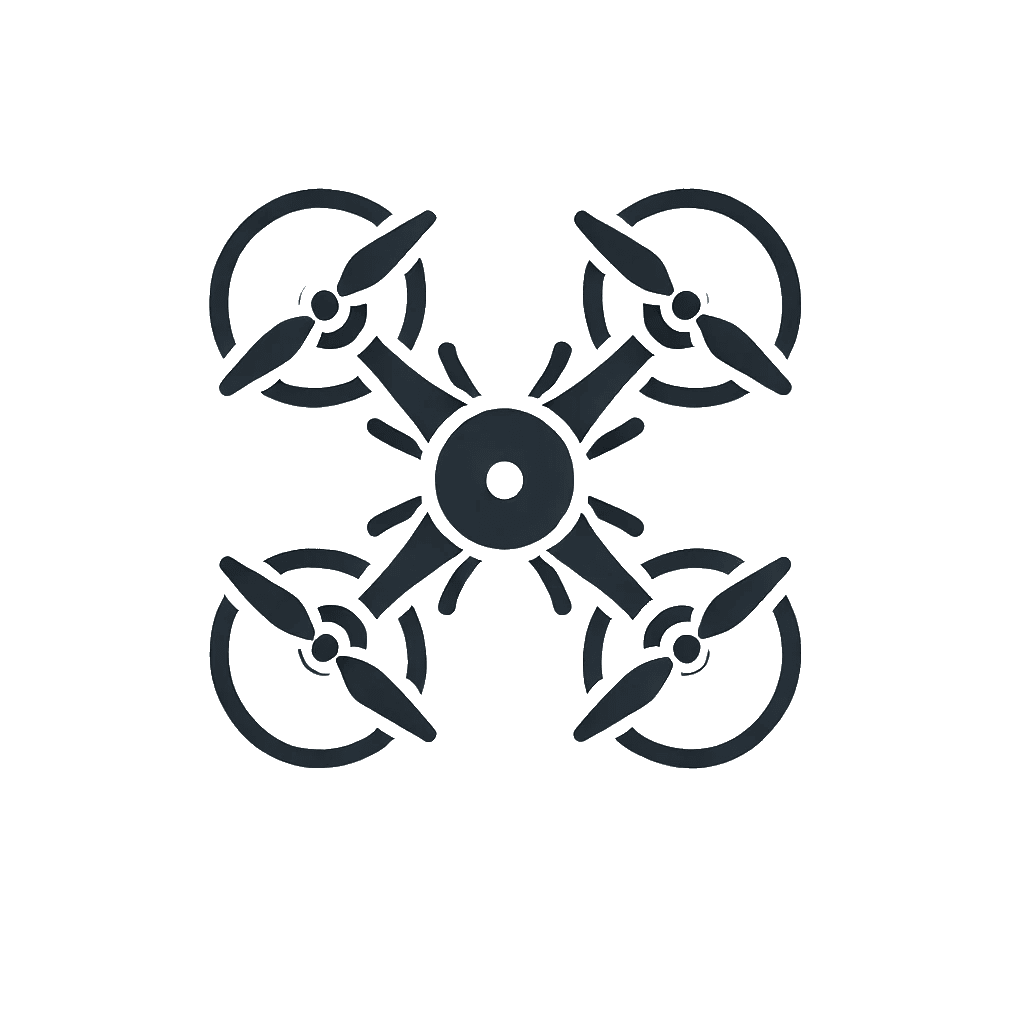
\includegraphics[width=1cm]{figures/drone_scheme.png}};
    }
    
    % Draw the connections
    \draw[dotted] (A) -- (B);
    \draw[dotted] (B) -- (C);
    % \draw[dotted] (B) -- (D);
    \draw[dotted] (D) -- (E);
    \draw[dotted] (E) -- (F);
    % \draw[dotted] (F) -- (G);
    
    % Add agent symbols as green circles
    \node[fill=green, circle, minimum size=7pt, inner sep=0pt] at (0.41,2.41) {};
    \node[fill=green, circle, minimum size=7pt, inner sep=0pt] at (2.41,2.41) {};
    \node[fill=green, circle, minimum size=7pt, inner sep=0pt] at (1.41,3.41) {};
    \node[fill=green, circle, minimum size=7pt, inner sep=0pt] at (3.41,3.41) {};
    \node[fill=green, circle, minimum size=7pt, inner sep=0pt] at (4.41,2.41) {};
    \node[fill=green, circle, minimum size=7pt, inner sep=0pt] at (5.41,3.41) {};
    \node[fill=green, circle, minimum size=7pt, inner sep=0pt] at (6.41,2.41) {};
    
    % Add blue circles to the left of some green circles
    \node[fill=blue, circle, minimum size=7pt, inner sep=0pt] at (0.11,2.41) {};
    \node[fill=blue, circle, minimum size=7pt, inner sep=0pt] at (2.11,2.41) {};
    \node[fill=blue, circle, minimum size=7pt, inner sep=0pt] at (3.11,3.41) {};
    \node[fill=blue, circle, minimum size=7pt, inner sep=0pt] at (5.11,3.41) {};
    
    % Add one additional circle to the left of an existing circle
    \node[fill=red, circle, minimum size=7pt, inner sep=0pt] at (4.11,2.41) {}; % Example: red circle added

    % Add the legend
    \node[fill=red, circle, minimum size=7pt, inner sep=0pt, label=right:{\small red agent}] at (0,1) {};
    \node[fill=blue, circle, minimum size=7pt, inner sep=0pt, label=right:{\small blue agent}] at (3,1) {};
    \node[fill=green, circle, minimum size=7pt, inner sep=0pt, label=right:{\small green agent}] at (6,1) {};
    
    \node at (1,0.5) {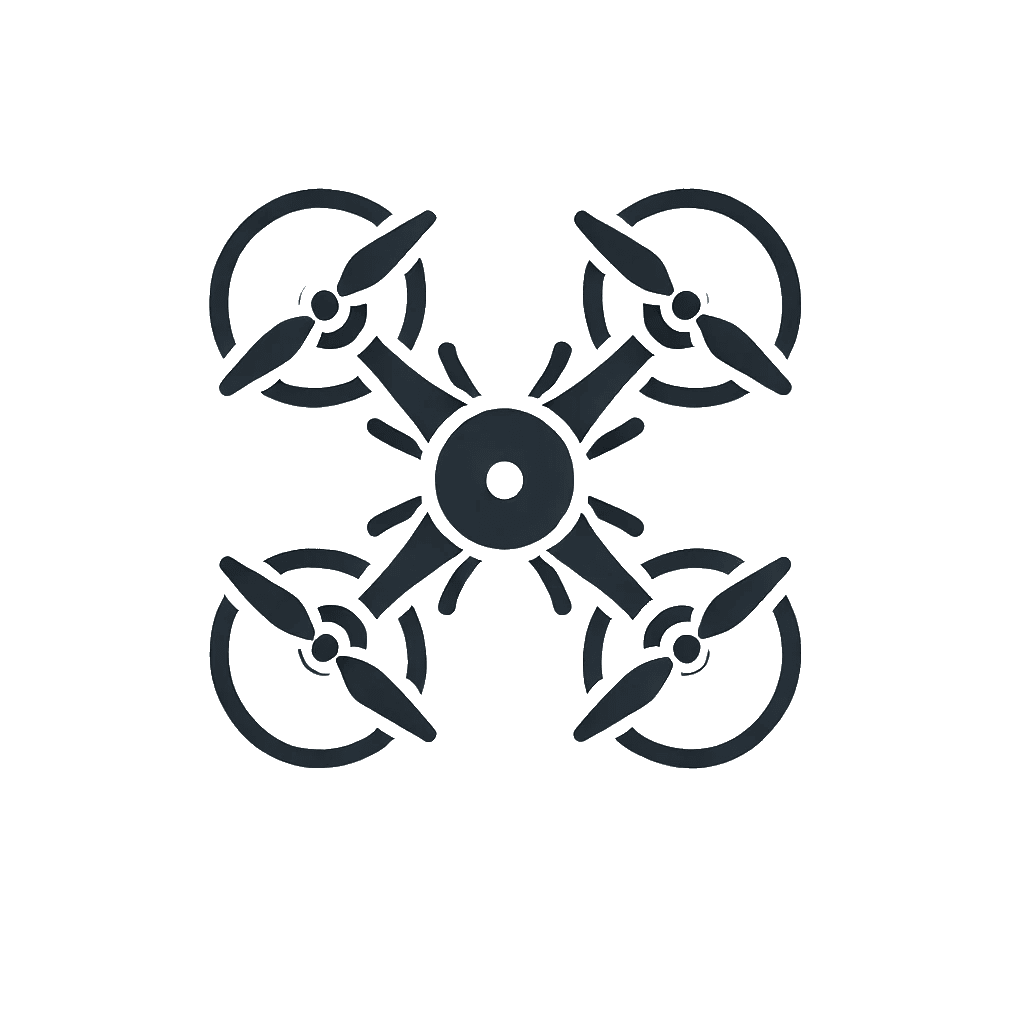
\includegraphics[width=1cm]{figures/drone_scheme.png}};
    \node[anchor=west] at (2,0.5) {\small drone};

    % Communication lines in legend
    \begin{scope}
        \draw[dotted] (4,0.5) -- (5,0.5);
        \node[anchor=west] at (5.1,0.5) {\small communication};
    \end{scope}
    
\end{tikzpicture}
    \caption{An illustrative view of the 3rd CAGE Challenge Scenario}\label{fig:cage_challenge}
\end{figure}

The scenario features three types of agents:
\begin{itemize}
    \item \textbf{Blue Agents (Defenders)}: Tasked with maintaining the security and functionality of the drone network. Their roles include controlling drones, preventing unauthorized access, and ensuring data integrity. They can perform actions such as \textit{RetakeControl}, \textit{RemoveOtherSessions}, and \textit{BlockTraffic}.
    \item \textbf{Red Agents (Attackers)}: Aim to compromise the drones to disrupt communication and control. They exploit vulnerabilities and can perform actions like \textit{ExploitDroneVulnerability}, \textit{SeizeControl}, and \textit{FloodBandwidth}.
    \item \textbf{Green Agents (Data Transfer)}: Simulate legitimate data communication to test the network's integrity, primarily through the \textit{SendData} action.
\end{itemize}

Each agent has a partial view of the environment, focusing on aspects such as network state, drone status, and communication observations. The reward structure for Blue agents is based on successful data transfers, control over drones, network security, and bandwidth management. Positive rewards are given for maintaining secure and functional communication, while penalties are imposed for losses in control, security breaches, and inefficient bandwidth usage.

This challenge emphasizes the need for advanced cybersecurity measures, efficient resource management, and effective multi-agent coordination, making it a relevant testbed for CoPRAHOM development.

\subsubsection{Organizational Models}

\begin{figure*}[h!]
    \centering
    


\tikzset{every picture/.style={line width=0.75pt}} %set default line width to 0.75pt        

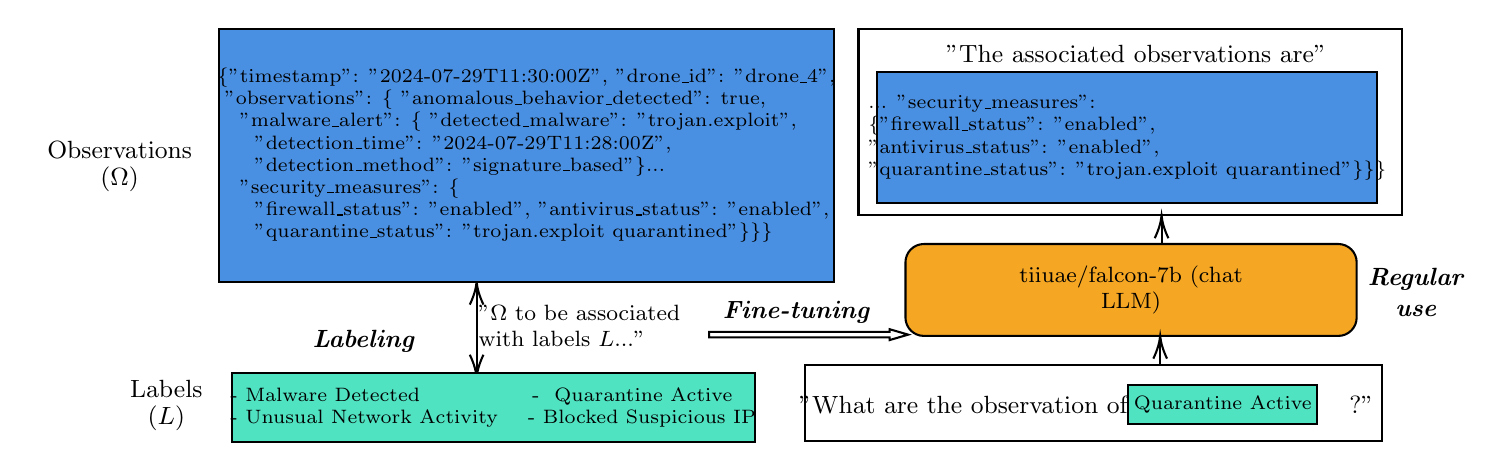
\begin{tikzpicture}[x=0.75pt,y=0.75pt,yscale=-1,xscale=1]
%uncomment if require: \path (0,1662); %set diagram left start at 0, and has height of 1662

%Rounded Rect [id:dp17386115134623514] 
\draw  [fill={rgb, 255:red, 245; green, 166; blue, 35 }  ,fill opacity=1 ] (424.61,402.58) .. controls (424.61,397.69) and (428.57,393.73) .. (433.46,393.73) -- (633.15,393.73) .. controls (638.04,393.73) and (642,397.69) .. (642,402.58) -- (642,429.15) .. controls (642,434.04) and (638.04,438) .. (633.15,438) -- (433.46,438) .. controls (428.57,438) and (424.61,434.04) .. (424.61,429.15) -- cycle ;
%Straight Lines [id:da8877910798706699] 
\draw    (547.33,451.83) -- (547.33,440) ;
\draw [shift={(547.33,438)}, rotate = 90] [color={rgb, 255:red, 0; green, 0; blue, 0 }  ][line width=0.75]    (10.93,-3.29) .. controls (6.95,-1.4) and (3.31,-0.3) .. (0,0) .. controls (3.31,0.3) and (6.95,1.4) .. (10.93,3.29)   ;
%Shape: Rectangle [id:dp44726237549140535] 
\draw   (376,452.18) -- (654,452.18) -- (654,488.66) -- (376,488.66) -- cycle ;
%Shape: Rectangle [id:dp2820683536345354] 
\draw   (402,290.27) -- (664,290.27) -- (664,379.64) -- (402,379.64) -- cycle ;
%Right Arrow [id:dp4162270206865013] 
\draw   (330,436.09) -- (417,436.09) -- (417,434.78) -- (425.91,437.39) -- (417,440) -- (417,438.7) -- (330,438.7) -- cycle ;
%Straight Lines [id:da8267677953106705] 
\draw    (548,393.83) -- (548,382) ;
\draw [shift={(548,380)}, rotate = 90] [color={rgb, 255:red, 0; green, 0; blue, 0 }  ][line width=0.75]    (10.93,-3.29) .. controls (6.95,-1.4) and (3.31,-0.3) .. (0,0) .. controls (3.31,0.3) and (6.95,1.4) .. (10.93,3.29)   ;
%Straight Lines [id:da6319519397458309] 
\draw    (218,456) -- (218,414) ;
\draw [shift={(218,412)}, rotate = 90] [color={rgb, 255:red, 0; green, 0; blue, 0 }  ][line width=0.75]    (10.93,-3.29) .. controls (6.95,-1.4) and (3.31,-0.3) .. (0,0) .. controls (3.31,0.3) and (6.95,1.4) .. (10.93,3.29)   ;
\draw [shift={(218,458)}, rotate = 270] [color={rgb, 255:red, 0; green, 0; blue, 0 }  ][line width=0.75]    (10.93,-3.29) .. controls (6.95,-1.4) and (3.31,-0.3) .. (0,0) .. controls (3.31,0.3) and (6.95,1.4) .. (10.93,3.29)   ;


% Text Node
\draw (68.5,471.5) node  [font=\footnotesize] [align=left] {\begin{minipage}[lt]{35.92pt}\setlength\topsep{0pt}
\begin{center}
{\small Labels ($\displaystyle L$)}
\end{center}

\end{minipage}};
% Text Node
\draw (372.5,426.5) node  [font=\small] [align=left] {\textit{\textbf{Fine-tuning}}};
% Text Node
\draw  [fill={rgb, 255:red, 74; green, 144; blue, 226 }  ,fill opacity=1 ]  (411,311) -- (652,311) -- (652,374) -- (411,374) -- cycle  ;
\draw (531.5,342.5) node  [font=\scriptsize] [align=left] {... "security\_measures":\\\{"firewall\_status": "enabled",\\"antivirus\_status": "enabled",\\"quarantine\_status": "trojan.exploit quarantined"\}\}\}};
% Text Node
\draw  [fill={rgb, 255:red, 80; green, 227; blue, 194 }  ,fill opacity=1 ]  (532,461.66) -- (623,461.66) -- (623,480.66) -- (532,480.66) -- cycle  ;
\draw (577.5,471.16) node  [font=\scriptsize] [align=left] {Quarantine Active};
% Text Node
\draw (536,302.25) node  [font=\footnotesize] [align=left] {{\small "The associated observations are"}};
% Text Node
\draw (671,417) node  [font=\small] [align=left] {\begin{minipage}[lt]{36.9pt}\setlength\topsep{0pt}
\begin{center}
\textit{\textbf{Regular}}\\\textit{\textbf{use}}
\end{center}

\end{minipage}};
% Text Node
\draw (512,471.16) node  [font=\footnotesize] [align=left] {{\small "What are the observation of \ \ \ \ \ \ \ \ \ \ \ \ \ \ \ \ \ \ \ \ \ \ \ \ \ ?"}};
% Text Node
\draw (46,356.32) node  [font=\footnotesize] [align=left] {\begin{minipage}[lt]{59.79pt}\setlength\topsep{0pt}
\begin{center}
{\small Observations ($\displaystyle \Omega $)}
\end{center}

\end{minipage}};
% Text Node
\draw (164,440.5) node  [font=\small] [align=left] {\textit{\textbf{Labeling}}};
% Text Node
\draw (267.5,433) node  [font=\footnotesize] [align=left] {{\footnotesize "$\displaystyle \Omega $ to be associated}\\{\footnotesize with labels $\displaystyle L$..."}};
% Text Node
\draw (533.3,415.86) node  [font=\footnotesize] [align=left] {\begin{minipage}[lt]{99.33pt}\setlength\topsep{0pt}
\begin{center}
tiiuae/falcon-7b (chat LLM)
\end{center}

\end{minipage}};
% Text Node
\draw  [fill={rgb, 255:red, 80; green, 227; blue, 194 }  ,fill opacity=1 ]  (100,456) -- (352,456) -- (352,489) -- (100,489) -- cycle  ;
\draw (226,472.5) node  [font=\scriptsize] [align=left] {\mbox{-} Malware Detected \ \ \ \ \ \ \ \ \ \ \ \ \ \ - \ Quarantine Active\\\mbox{-} Unusual Network Activity \ \ \ - Blocked Suspicious IP};
% Text Node
\draw  [fill={rgb, 255:red, 74; green, 144; blue, 226 }  ,fill opacity=1 ]  (94,290) -- (390,290) -- (390,412) -- (94,412) -- cycle  ;
\draw (242,351) node  [font=\scriptsize] [align=left] {\{"timestamp": "2024-07-29T11:30:00Z", "drone\_id": "drone\_4",\\ \ "observations": \{ "anomalous\_behavior\_detected": true,\\ \ \ \ "malware\_alert": \{ "detected\_malware": "trojan.exploit",\\ \ \ \ \ \ "detection\_time": "2024-07-29T11:28:00Z",\\ \ \ \ \ \ "detection\_method": "signature\_based"\}...\\ \ \ \ "security\_measures": \{\\ \ \ \ \ \ "firewall\_status": "enabled", "antivirus\_status": "enabled",\\ \ \ \ \ \ "quarantine\_status": "trojan.exploit quarantined"\}\}\}};


\end{tikzpicture}
    \caption{LLM training and use for applying CoPRAHOM to the 3rd CAGE Challenge}\label{fig:llm_process}
\end{figure*}


We implemented and evaluated two organizational models using the \textit{MASCARA-$\mathcal{M}OISE^+$} model and tailored for the CybORG 3rd CAGE Challenge environment:

The "\textbf{Active Defense}" model implements proactive measures for threat anticipation, detection, and mitigation. It focuses on maintaining network security and functionality through predefined three roles:
%
\textit{Threat Assessor}: Monitors the network, identifying potential threats using advanced analytics;
\textit{Response Strategist}: Oversees response strategies to neutralize identified threats;
\textit{Network Guardian}: Ensures network integrity and availability by implementing security measures.
%
This model also includes the \textit{Proactive Threat Detection} mission which contains goals for early detecting of threats using predictive analytics.

The "\textbf{Suspect Isolation}" emphasizes identifying and isolating compromised network elements to contain threats through three roles:
%
\textit{Anomaly Detector}: Identifies anomalies indicating potential breaches;
\textit{Isolation Specialist}: Isolates compromised systems to prevent threat spread;
\textit{Incident Responder}: Coordinates response and executes isolation protocols.
%
This model also includes the \textit{Compromised Drone Detection} mission which contains goals for detecting compromised drones and isolating them from the network as well as the \textit{Containment and Isolation} mission which contains goals for isolating compromised systems from the network.

Additionally, we established a non MASCARA-based model called "\textbf{Manual}" based on our empirical understanding of the environment, serving as a baseline model.
We also considered a totally non-constrained case as "\textbf{Free}" to serve as a regular MARL reference for comparison.


\subsubsection{Experimental Procedure}

We trained each organizational model using the \textit{CoPRAHOM Wrapper} with the provided \textit{CybORG} simulator. The wrapper integrates organizational specifications and constraints during learning, enabling agents to learn and adapt their behavior based on predefined roles and missions.

We selected the MAPPO algorithm for its proven efficiency in cooperative multi-agent environments without the need for domain-specific algorithmic modifications or architectures~\cite{Yu2022}. We used the MAPPO-implemented algorithm model provided by MARLlib. Specifically, we configured the MAPPO model with a two-layer MLP network, comprising 128 neurons in the first layer and 256 in the second, optimized using Adam with a learning rate of 0.0003. These configurations were chosen based on preliminary experiments and available MARLlib fine-tuned hyper-parameters models. We launched the training over 70 iterations (each consisting of 128 episodes) in a Centralized Learning and Decentralized Execution manner.\\

To train the LLM with \texttt{ol\_mngr}, we explored the environment manually, step-by-step, using controlled policies. This approach allowed the agent to encounter the most relevant situations for detecting and mitigating malware programs. For example, these include situations where an agent receives messages we think to be suspicious or situations where an agent receives a confirmation to kill a process. Throughout this exploration, we collected, displayed (as JSON or graph representation), interpreted, and labeled several observations to a few keywords. This labeling helps in easily identifying collective behaviors based on visual observations, enabling better control of agents' actions. The whole training and use process is summarized in \autoref{fig:llm_process}

\subsubsection{Evaluation metrics}

We used various metrics to measure the impact of CoPRAHOM during and after training:
\begin{itemize}
    \item \textbf{Scalability}: Assesses the ability to manage a growing number of agents and obstacles based on computational resource usage.
    \item \textbf{Convergence Time}: The number of episodes required for the algorithm to reach a stable solution. Shorter convergence times indicate faster learning.
    \item \textbf{Standard Deviation}: Indicates the variability in the rewards obtained by the agents. A lower standard deviation signifies more consistent performance and potentially more stable organization.
    \item \textbf{Average Reward}: The mean reward obtained per episode reflects the overall performance of the algorithm.
    \item \textbf{Constraint Respect}: Assesses how well the agents adhere to the given organizational constraints. %It is calculated as the inverse of the number of times the constraints are not satisfied. High constraint respect means that the agents are effectively following the rules.
\end{itemize}

We also included these two Cyberdefense-specific metrics:
\begin{itemize}
    \item \textbf{Average Percentage of Infected Drones by Malware}: Measures the proportion of drones infected by malware during the simulation.
    \item \textbf{Average Percentage of Successful Malware Attacks}: Indicates the success rate of attacks on the drone swarm.
\end{itemize}

\subsubsection{Criteria for validation}

Using the aforementioned metrics, we defined criteria to assess the enhancement in Cyberdefense provided by CoPRAHOM compared to regular MARL learning, particularly focusing on the "Active Defense" model. The criteria are:

\begin{itemize}
    \item $\mathbf{C_1}$: We expect to manually notice some collective strategies, such as isolating suspicious activities or coordinating defensive maneuvers.
    \item $\mathbf{C_2}$: We expect to see faster convergence in the "Active Defense" or "Suspect Isolation" models than in the "Free" case, and "Manual" one to show a constant learning curve.
    \item $\mathbf{C_3}$: We expect higher rewards in the "Active Defense" or "Suspect Isolation" models compared to the "Free" case.
    \item $\mathbf{C_{4}}$: We expect the standard deviation to decrease from "Free" to "Active Defense" or "Suspect Isolation" models and from "Active Defense" or "Suspect Isolation" models to the "Manual" model, since agents are increasingly more constrained in their behavior.
    \item $\mathbf{C_{5}}$: We expect the constraint respect to be fully covered in \textit{correct} and \textit{correct\_policy} modes but not in the \textit{penalize} mode.
    \item $\mathbf{C_{6}}$: We expect the scalability to be handled in all of the cases.
    \item $\mathbf{C_7}$: Lower average percentage of infected drones in "Active Defense" or "Suspect Isolation" models compared to the "Free" case.
    \item $\mathbf{C_8}$: Lower average percentage of successful malware attacks in "Active Defense" or "Suspect Isolation" models compared to the "Free" case.

\end{itemize}

\subsection{Results and Discussion}\label{sec:results_and_discussion}

\autoref{fig:learning_curves} illustrates the learning curves for the "Suspect Isolation", "Active Defensive", and "Manual" models, indicating their convergence rates over training episodes.
\autoref{tab:metrics_comparison} summarizes the convergence time during training as well as the average rewards, standard deviation, average infection drone, and average malware attack achieved models after training over a dozen episodes.

\begin{figure}[ht]
    \centering
    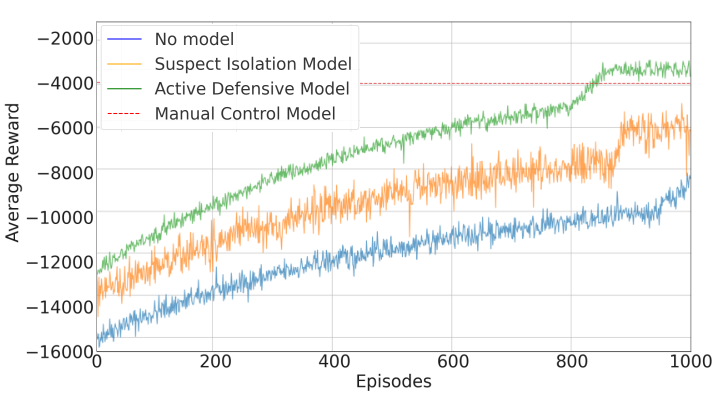
\includegraphics[width=1\linewidth]{figures/learning_curves.png}
    \caption{Learning curves for \textit{Free}, \textit{Suspect Isolation}, \textit{Active Defense}, \textit{Manual} using the \textit{correct\_policy} mode}
    \label{fig:learning_curves}
\end{figure}

\begin{table*}[t]
    \centering
    \setlength{\tabcolsep}{4.5pt}
    \caption{Comparison of models and constraint modes with respect to metrics.}
    \label{tab:metrics_comparison}
    \begin{tabular}{lcccccccccccc}
                               & {Free}      & \multicolumn{3}{c}{Suspect Isolation} & \multicolumn{3}{c}{Active Defense} & {Manual}                                                       \\
        % \cline{2-13}
        Metric                 &             & Penalize                              & Correct                              & Correct\_Policy  & Penalize & Correct  & Correct\_Policy &             \\
        \midrule
        Average Reward         & -8727.49    & -5900.00                              & -6085.12                             & -6088.00         & -3055.36 & -3100.00 & -3060.00        & -3906.00    \\
        Standard Deviation     & 138.00      & 2148.0                               & 2027.0                              & 2018.00          & 962.   & 940.00   & 945.00          & 570.33     \\
        Scalability            & Medium      & High                                  & Medium                               & Medium  & High     & Medium   & Medium & Medium      \\
        Convergence Time & >1000 & 1000 & 950 & 950 & 800 & 850 & 850 & $\emptyset$ \\
        Constraint Respect     & $\emptyset$ & Low                                   & High                                 & High             & Medium   & High     & High            & $\emptyset$      \\
        Avg. Inf. Drones (\%)  & 61.0        & 43.0                                  & 30.0                                 & 23.0             & 24.0     & 25.0     & 20.0            & 40.0        \\
        Avg. Malware Att. (\%) & 72.0        & 55.0                                  & 52.0                                 & 45.0             & 38.0     & 45.0     & 40.0            & 51.0        \\
    \end{tabular}
\end{table*}

The organizational models effectively influenced drone behavior in the CybORG CAGE Challenge 3 environment. The "Suspect Isolation" model demonstrated effective identification and isolation of drones exhibiting suspicious activities, enhancing overall security. This model ensured that potential threats were quickly identified and neutralized, preventing the spread of malicious activities within the drone swarm ($\mathbf{C_1}$).

\autoref{fig:learning_curves} provides a comprehensive view of the learning curves for each model. The "Free" model (blue) exhibited the slowest convergence and the lowest average rewards. Moreover, it also shows a low variability in rewards indicating that agents are slowly trained with limited changes at each step. This result is expected as the learning rate for MAPPO is relatively low.

In contrast, the "Suspect Isolation" model (orange) showed faster convergence and higher average rewards compared to the "Free" model. Yet, the increased variability (compared to "Free") suggests that since agents are forced/enticed to satisfy some rules to identify and isolate suspicious activities, their policies may require time to get used to these rules to reach a more stable behavior.

The "Active Defense" model (green) exhibited the highest average rewards and the fastest convergence among all models. The steadily increasing rewards demonstrate the efficiency of proactive defense strategies implemented by the agents. This model showed the greatest improvement in performance, underscoring the benefits of using structured organizational constraints to guide agent behavior. The "Active Defense" model also shows a lower variability in rewards compared to "Suspect Isolation" model but higher compared to the "Free" model. This suggests that while agents are still adapting to the constraints, their possible behaviors is more limited in "Active Defense" model than in "Suspect Isolation" model.

The "Manual" model (red dashed line) served as a baseline for comparison. It performed better than the "Free" and "Suspect Isolation" models but was outperformed by the "Active Defense" model. This can be explained as the manual control strategy, although effective, lacked the adaptability and efficiency provided by the learned organizational models.

From a quantitative perspective, the metrics also provide evidence for the advantages of applying organizational constraints. As illustrated in \autoref{fig:learning_curves}, in the constrained policy case, agents exhibited faster convergence compared to the "Free" model across all modes. This confirms that organizational constraints can accelerate learning ($\mathbf{C_2}$). The manually crafted policy case achieved immediate convergence, as expected, due to the absence of learning.

The average reward metrics reveal that agents guided by the "Suspect Isolation" model consistently outperformed those in the "Free" model, achieving higher rewards ($\mathbf{C_3}$). This indicates that organizational constraints not only improve learning efficiency but also enhance overall performance. The manually crafted policies consistently achieved the highest rewards, highlighting the efficiency of well-defined constraints.

Concerning constrained models, the standard deviation in \autoref{tab:metrics_comparison} decreased progressively from the less constrained model such as "Suspect Isolation" to the most constrained model such "Active Defense" ($\mathbf{C_4}$). This reduction in variability suggests that organizational constraints contribute to more stable and consistent agent behavior.

The criterion of constraint respect was fully met in the \textit{correct} and \textit{correct\_policy} modes, but not in the \textit{penalize} mode ($\mathbf{C_5}$). This demonstrates that while agents can learn to follow constraints effectively, the mode of constraint integration plays a crucial role. In our evaluation, the \textit{correct} and \textit{correct\_policy} modes demonstrated full adherence to organizational constraints, as evidenced by zero deviations in agent behavior from prescribed roles and missions. In contrast, the \textit{penalize} mode showed occasional deviations, particularly under high lesser constrained models such as "Suspect Isolation". This suggests that agents occasionally prioritize reward maximization over strict constraint adherence. Further analysis for penalization strategies would improve compliance.

Scalability, assessed by evaluating the system's performance under increased numbers of agents and obstacles, was effectively managed across all models ($\mathbf{C_6}$). Particularly, the \textit{penalize} mode showed superior scalability due to built-in efficient computation of policy updates, unlike the \textit{correct} and \textit{correct\_policy} modes that require aside correction functions.

Both "Active Defense" and "Suspect Isolation" models impacted the metrics for "Average Percentage of Infected Drones" and "Average Percentage of Successful Malware Attacks" ($\mathbf{C_7}$ and $\mathbf{C_8}$). Yet, it is important to note these two metrics are not directly related to the overall reward, since they are calculated separately. The "Active Defense" model achieved the best results, reducing the percentage of infected drones to 23\% and successful malware attacks to 38\%. This significant reduction, compared to the 61\% infection rate and 72\% success rate in the "Free" model, demonstrates the efficacy of proactive defensive strategies in preventing malware propagation and successful attacks. The "Suspect Isolation" model also showed lower infection and attack success rates than the "Free" model.

% These findings underscore the importance of implementing structured organizational constraints and proactive defense mechanisms within autonomous systems. The integration of $\mathcal{M}OISE^+$ organizational models within the MARL framework, as demonstrated by CoPRAHOM, proves to significantly enhance the efficiency and coordination of autonomous cyber defense agents. The experimental results highlight that structured organizational constraints not only improve agent performance and stability but also ensure that their behavior aligns with mission objectives and cybersecurity goals.

% The results suggest that further refinement of organizational specifications and incorporation of more sophisticated rules and protocols could yield even greater enhancements in agent behavior and coordination. This ongoing development promises to bolster the resilience and robustness of cyber defense strategies against increasingly sophisticated threats.
% However, CoPRAHOM's generalizability to different real-world Cyberdefense scenarios, such as IoT security or industrial control systems, may require adjustments in organizational specifications and policy constraints. Future work should explore these adaptations to validate CoPRAHOM's broad applicability.

\subsection{Conclusion}\label{sec:conclusion}

Our contribution is motivated by the high cost of designing Cyberdefense Multi-Agent Systems (MAS) in various scenarios, particularly when dealing with constantly evolving threats. To address this issue, we propose a dedicated algorithm called CoPRAHOM, that leverages Multi-Agent Reinforcement Learning (MARL) according to organizational specifications. CoPRAHOM ensures that some constraints are met in the agents' behavior, helping in the monitoring and understanding of the trained agents.

CoPRAHOM was evaluated using our proposed PoC implementation for the 3rd CAGE Challenge, a cooperative Cyberdefense drone swarm scenario designed to limit/eliminate malware programs and their impact. We established various organizational models, ranging from minimally constrained to fully constrained ones. We conducted an evaluation of the emergent, fine-tuned, or predefined collective strategies based on performance criteria during and after the training.

The results indicate that constraints-balanced models like the "Active Defensive Model" achieve a significant tradeoff between constraints and autonomous learning. This model employs straightforward predefined rules to detect and address threats when observations are unambiguous, while still allowing the agent to learn how to respond in other scenarios.

In addition to constraining agents according to organizational specifications, we aim to consider explainability mechanisms to understand newly learned organizational patterns. The idea of iterative improvement between training and explainability could greatly benefit from hierarchical learning, which helps characterize and bring out strategies during learning.
%Furthermore, while the initial results obtained with LLM show it as a promising complementary tool for CoPRAHOM, it may also offer new avenues for explaining collective behavior, especially in Cyberdefense scenarios where most networked environments are not visually or intuitively representable.

% Ultimately, we also aim to improve the applicability of PRAHOM by developing dedicated interfaces built around PRAHOM making it more accessible to industrial and research contexts.

